% !TeX root = ../../Book3.tex
% 纲要标题：### 6.1 长度与能量的变分
% 纲要位置：几何学计划纲要.md，第 2328 行。
% 正文状态：初稿；尚未正式审核。

% 纲要内容开始
% 
% * 变分场和协变导数交换
% * 第一变分及端点项
% * 第二变分和曲率项
% * 固定端点与自由端点的区别
% 
% 纲要内容结束

\section{长度与能量的变分}
\label{g3:sec:0601}

第二章用法邻域比较曲线长度，得到短测地线的极小性。现在固定一条曲线，把它向附近推开，考察长度先怎样变化、再怎样弯曲。一次变化检验曲线是否驻定，二次变化检验驻定曲线附近是否存在下降方向。端点是否允许移动会改变这两次计算的边界项，因而必须从一开始就说明允许哪些变分。

\subsection{变分场和协变导数交换}
\label{g3:subsec:0601:01}

设 \((M,g)\) 为光滑无边界黎曼流形，\(a<b\)。对光滑曲线 \(\gamma:[a,b]\to M\)，一个满足 \(F(0,t)=\gamma(t)\) 的光滑映射
\[
	F:(-\varepsilon,\varepsilon)\times[a,b]\longrightarrow M
\]
称为它的\term[quxian bianfen]{变分}[variation]。参数 \(s\) 选择附近的曲线，参数 \(t\) 沿每条曲线前进。记
\[
	T=\partial_tF,\qquad S=\partial_sF,\qquad V(t)=S(0,t).
\]
沿 \(\gamma\) 的向量场 \(V\) 称为\term[bianfen chang]{变分场}[variational vector field]。若 \(F(s,a),F(s,b)\) 分别恒等于 \(\gamma(a),\gamma(b)\)，就称变分固定端点。也允许 \(F\) 连续且在一个共同的有限 \(t\)-分割上分片光滑；每片均光滑到边界，各片的 \(s\)-导数在接缝处相同。这使变分场连续，而 \(D_tV\) 可以有跳跃。

\begin{figure}[htbp]
	\centering
	% !TeX root = ../Book3.tex
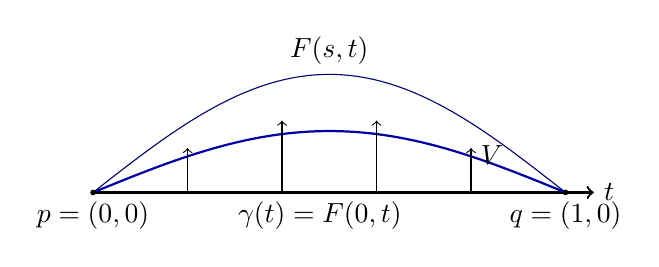
\begin{tikzpicture}[x=6cm,y=1.2cm]
	\draw[thick,->] (0,0)--(1.06,0) node[right] {\(t\)};
	\draw[blue!65!black,thick,domain=0:1,samples=60] plot (\x,{0.65*sin(180*\x)});
	\draw[blue!45!black,domain=0:1,samples=60] plot (\x,{1.25*sin(180*\x)});
	\foreach \x in {0.2,0.4,0.6,0.8}{
		\draw[->] (\x,0)--(\x,{0.8*sin(180*\x)});
	}
	\fill (0,0) circle[x radius=.006,y radius=.03];
	\fill (1,0) circle[x radius=.006,y radius=.03];
	\node[below] at (0,0) {\(p=(0,0)\)};
	\node[below] at (1,0) {\(q=(1,0)\)};
	\node[below] at (.48,0) {\(\gamma(t)=F(0,t)\)};
	\node[above] at (.5,1.25) {\(F(s,t)\)};
	\node[right] at (.8,.4) {\(V\)};
\end{tikzpicture}

	\caption{Euclid 平面上的固定端点变分 \(F(s,t)=(t,s\sin\pi t)\)。箭头表示沿水平基曲线的变分场 \(V=(0,\sin\pi t)\)，两端的场为零。}
	\label{g3:fig:fixed-endpoint-variation}
\end{figure}

沿 \(F\) 的协变导数使用拉回切丛。在任一坐标图中，若 \(Z=Z^k\partial_k|_F\)，则
\[
	(D_tZ)^k=\partial_tZ^k+\Gamma^k_{ij}(F)T^iZ^j,
	\qquad (D_sZ)^k=\partial_sZ^k+\Gamma^k_{ij}(F)S^iZ^j.
\]
因此这些运算不要求 \(F\) 是浸入，也不要求变分曲线互不相交。第二章证明 Gauss 引理时已经用过这种计算；现在还要交换两次协变导数。

\begin{proposition}\label{g3:prop:variation-commutation}
	设 \(F\) 是光滑无边界黎曼流形中的光滑二参数映射，\(T=\partial_tF\)、\(S=\partial_sF\)，\(Z\) 为沿 \(F\) 的光滑向量场。对 Levi-Civita 联络及本卷曲率约定，有
	\begin{equation}\label{g3:eq:variation-commutation}
		D_sT=D_tS,\qquad D_sD_tZ-D_tD_sZ=R(S,T)Z.
	\end{equation}
\end{proposition}
\begin{proof}
	第一式由 \(\partial_s\partial_tF^k=\partial_t\partial_sF^k\) 与 \(\Gamma^k_{ij}=\Gamma^k_{ji}\) 得到，即\eqref{g3:eq:mixed-variation-derivatives}。对第二式展开上面的两次导数，含 \(\partial_s\partial_tZ\)、一阶 \(Z\) 导数以及 \(\partial_sT^i-\partial_tS^i\) 的项相消。余项为
	\[
		\bigl(\partial_i\Gamma^k_{j\ell}-\partial_j\Gamma^k_{i\ell}
		+\Gamma^k_{ir}\Gamma^r_{j\ell}-\Gamma^k_{jr}\Gamma^r_{i\ell}\bigr)
		S^iT^jZ^\ell.
	\]
	由\eqref{g3:eq:curvature-coordinate-components}，这正是 \(R(S,T)Z\) 的第 \(k\) 个分量。
\end{proof}

任意沿 \(\gamma\) 的光滑场都能成为变分场。事实上，第二章的指数映射在零截面附近光滑；\([a,b]\) 紧，故对充分小的共同 \(s\)，可定义
\begin{equation}\label{g3:eq:exponential-field-variation}
	F(s,t)=\exp_{\gamma(t)}(sV(t)).
\end{equation}
由 \((\mathrm d\exp_x)_0=I\)，其变分场为 \(V\)。若 \(V(a)=V(b)=0\)，这个变分固定端点。连续分片光滑场也由同一公式实现为上述分片光滑变分。这里的紧性只涉及所给曲线的参数区间，无须假设整个 \(M\) 完备。

\subsection{第一变分及端点项}
\label{g3:subsec:0601:02}

对分片光滑曲线 \(c:[a,b]\to M\)，定义其\term[quxian nengliang]{能量}[energy]和长度
\begin{equation}\label{g3:eq:curve-energy-length}
	E(c)=\frac12\int_a^b|\dot c|^2\,\mathrm dt,
	\qquad L(c)=\int_a^b|\dot c|\,\mathrm dt.
\end{equation}
\symidx{\(E(c)\)：曲线能量}
长度在保向重参数化下不变，能量还记录行进速度。在固定区间上，Cauchy--Schwarz 不等式给出
\begin{equation}\label{g3:eq:energy-length-inequality}
	L(c)^2\le2(b-a)E(c),
\end{equation}
等号当且仅当速度长度几乎处处为同一个常数。特别地，若连接两端点的常速最短测地线 \(\gamma\) 存在，则
\[
	E(c)\ge \frac{L(c)^2}{2(b-a)}
	\ge\frac{d(\gamma(a),\gamma(b))^2}{2(b-a)}=E(\gamma).
\]
等号要求曲线同时最短且常速。使用能量可以保留测地线参数，又避开长度被积式在零速度处不可微的问题。

\begin{theorem}[第一变分]\label{g3:thm:curve-first-variation}
	设 \(F\) 是光滑无边界黎曼流形中光滑曲线 \(\gamma:[a,b]\to M\) 的光滑变分，\(V=\partial_sF|_{s=0}\)、\(T=\dot\gamma\)。则
	\begin{equation}\label{g3:eq:energy-first-variation}
		\left.\frac{\mathrm d}{\mathrm ds}E(F(s,\cdot))\right|_{s=0}
		=[\langle V,T\rangle]_a^b-\int_a^b\langle V,D_tT\rangle\,\mathrm dt.
	\end{equation}
	若 \(\gamma\) 正则，即 \(|T|>0\)，令 \(U=T/|T|\)，则
	\begin{equation}\label{g3:eq:length-first-variation}
		\left.\frac{\mathrm d}{\mathrm ds}L(F(s,\cdot))\right|_{s=0}
		=[\langle V,U\rangle]_a^b-\int_a^b\langle V,D_tU\rangle\,\mathrm dt.
	\end{equation}
\end{theorem}
\begin{proof}
	度量相容性和\cref{g3:prop:variation-commutation}给出
	\[
		\partial_s\tfrac12|\partial_tF|^2
		=\langle D_sT,T\rangle=\langle D_tS,T\rangle.
	\]
	对紧区间求导积分并分部积分，得到第一式。正则曲线的速度在紧区间上有正下界，所以充分小的变分也正则；此时
	\(\partial_s|T|=\langle D_tS,T/|T|\rangle\)。再次分部积分即得第二式。
\end{proof}

\begin{corollary}\label{g3:cor:energy-critical-geodesic}
	光滑无边界黎曼流形中的光滑曲线，在所有固定端点光滑变分下能量一阶导数为零，当且仅当它是仿射参数测地线。正则曲线在所有这样的变分下长度一阶导数为零，当且仅当它的弧长参数化是测地线。
\end{corollary}
\begin{proof}
	端点项为零。若第一式对所有端点为零的场 \(V\) 消失，取非负紧支函数 \(\chi\) 并用 \(V=\chi D_tT\)，得到 \(\int\chi|D_tT|^2=0\)，所以 \(D_tT=0\)。反向由公式直接成立。长度的情形以 \(D_tU\) 替代 \(D_tT\)，得到 \(D_tU=0\)。因为弧长 \(\ell\) 满足 \(\mathrm d\ell/\mathrm dt=|T|>0\)，这等价于 \(D_\ell U=0\)。
\end{proof}

对分片光滑的基曲线，逐片分部积分还会在每个内节点 \(t_i\) 出现项
\begin{equation}\label{g3:eq:energy-corner-terms}
	\langle V(t_i),T(t_i^-)-T(t_i^+)\rangle.
\end{equation}
允许独立移动节点后，能量驻定要求这些速度跳跃全部为零。长度公式则用单位切向量 \(U\) 的跳跃；它排除角点，但不要求两侧速度大小相等。这与第二章最短曲线可以按弧长参数化为光滑测地线的结论相符。

\subsection{第二变分和曲率项}
\label{g3:subsec:0601:03}

以下在仿射参数测地线处求二次变化。记 \(V'=D_tV\)，并令
\[
	A(t)=(D_sS)(0,t).
\]
\(A\) 是各条 \(s\)-曲线的协变加速度，通常并不为零。一次变分只看 \(V\)；若端点可动，二次变分还会看到端点轨迹的加速度。

\begin{theorem}[能量第二变分]\label{g3:thm:energy-second-variation}
	设 \(\gamma:[a,b]\to M\) 为光滑无边界黎曼流形中的仿射参数测地线，\(F\) 为它的光滑变分，\(V=\partial_sF|_0\)、\(A=D_s\partial_sF|_0\)、\(T=\dot\gamma\)。则
	\begin{equation}\label{g3:eq:energy-second-variation}
		E''(0)=\int_a^b\bigl(|V'|^2-\langle R(V,T)T,V\rangle\bigr)\,\mathrm dt
		+[\langle A,T\rangle]_a^b.
	\end{equation}
	若变分固定端点，最后一项为零。若变分仅沿一个共同有限分割分片光滑，且变分场连续，同式仍按各片积分成立。
\end{theorem}
\begin{proof}
	在变分上对 \(E'(s)=\int\langle D_tS,T\rangle\) 再求导，得
	\[
		E''(0)=\int_a^b\bigl(\langle D_sD_tS,T\rangle+|D_tS|^2\bigr)\big|_{s=0}\,\mathrm dt.
	\]
	交换公式将第一项写成 \(\langle D_tA+R(V,T)V,T\rangle\)。由于 \(D_tT=0\)，对 \(D_tA\) 分部积分只留下端点项。\cref{g3:prop:curvature-symmetries}的斜伴随性质给出
	\[
		\langle R(V,T)V,T\rangle=-\langle R(V,T)T,V\rangle,
	\]
	于是得到所述公式。固定端点时，端点的整条 \(s\)-曲线为常曲线，故 \(A(a)=A(b)=0\)。在分片情形，各接缝处的 \(A\) 连续，基曲线的 \(T\) 也连续，因此内节点的边界项相消。
\end{proof}

当 \(T\) 为单位向量且 \(V\perp T\) 时，曲率项为 \(K(V,T)|V|^2\)。正曲率减小二次变化，负曲率增大二次变化。这是随后共轭点与曲率比较出现相反效应的具体原因。

\ProseParagraphBreak

固定端点时，二次变化只取决于 \(V\)，与实现它的变分的二阶数据无关。极化得到对称双线性形式
\begin{equation}\label{g3:eq:index-form-introduction}
	I_\gamma(V,W)=\int_a^b\bigl(\langle V',W'\rangle
	-\langle R(V,T)T,W\rangle\bigr)\,\mathrm dt.
\end{equation}
曲率对称性保证 \(V\mapsto R(V,T)T\) 自伴，故这个形式确实对称。在固定端点的二参数变分中，混合二阶导数就是 \(I_\gamma(V,W)\)：可把前一公式用于参数平面中每条直线，再由极化恒等式恢复混合项。\secref{g3:sec:0603}将把它作为指标形式系统研究。

\begin{theorem}[长度第二变分]\label{g3:thm:length-second-variation}
	设 \(\gamma:[a,b]\to M\) 为光滑无边界黎曼流形中的单位速测地线，\(F\) 为光滑变分，\(V,A,T\) 如前一定理。令 \(V^\perp=V-\langle V,T\rangle T\)，则
	\begin{align}
		L''(0)&=\int_a^b\bigl(|V'|^2-\langle V',T\rangle^2
		-\langle R(V,T)T,V\rangle\bigr)\,\mathrm dt
		+[\langle A,T\rangle]_a^b\notag\\
		&=I_\gamma(V^\perp,V^\perp)+[\langle A,T\rangle]_a^b.
		\label{g3:eq:length-second-variation}
	\end{align}
\end{theorem}
\begin{proof}
	令 \(q(s,t)=|\partial_tF|^2\)。在 \(s=0\) 处 \(q=1\)，故
	\[
		\partial_s^2\sqrt q=\tfrac12\partial_s^2q-\tfrac14(\partial_sq)^2.
	\]
	第一项积分是能量第二变分，而 \(\partial_sq|_0=2\langle V',T\rangle\)，得到第一行。写 \(V=fT+V^\perp\)，利用 \(D_tT=0\) 可得 \(V'=f'T+(V^\perp)'\)，其中后项仍垂直于 \(T\)。又因 \(R(T,T)=0\) 及 \(R(V^\perp,T)T\perp T\)，曲率项也只看 \(V^\perp\)，于是得到第二行。
\end{proof}

例如在 Euclid 空间中取单位直线段 \(\gamma\)，令 \(f(a)=f(b)=0\)。变分 \(F(s,t)=\gamma(t+sf(t))\) 在小 \(s\) 时只是重参数化，故长度恒定；其变分场是 \(V=fT\)，能量二次变化却为 \(\int_a^b(f')^2\)。长度的切向零方向来自参数自由度，不能将这些方向误认为几何上的共轭方向。

\subsection{固定端点与自由端点的区别}
\label{g3:subsec:0601:04}

现在允许起点在光滑嵌入子流形 \(P\) 内移动、终点在光滑嵌入子流形 \(Q\) 内移动。允许的场满足
\[
	V(a)\in T_{\gamma(a)}P,\qquad V(b)\in T_{\gamma(b)}Q.
\]
这些条件也足以实现变分。为说明这一点，在 \(P,Q\) 内选端点曲线 \(p(s),q(s)\)，其初速度分别是 \(V(a),V(b)\)。先用\eqref{g3:eq:exponential-field-variation}，再在指数映射的输入中加入两端的修正：用沿 \(\gamma\) 的平行运输，把
\[
	\eta_a(s)=\exp_{\gamma(a)}^{-1}p(s)-sV(a),\qquad
	\eta_b(s)=\exp_{\gamma(b)}^{-1}q(s)-sV(b)
\]
分别延到两端的短邻域，并乘以在相应端点为1、另一端附近为0的光滑截断函数。因为 \(\eta_a,\eta_b=O(s^2)\)，修正不改变变分场，却使端点恰落在 \(P,Q\) 上。这个构造也适用于连续分片光滑场。

\begin{proposition}\label{g3:prop:submanifold-endpoint-variation}
	设 \(P,Q\) 为光滑无边界黎曼流形 \((M,g)\) 的光滑嵌入子流形。光滑曲线 \(\gamma:[a,b]\to M\) 的两端分别在 \(P,Q\) 上。它在所有端点留在 \(P,Q\) 的变分下能量驻定，当且仅当它是测地线，且
	\[
		\dot\gamma(a)\perp T_{\gamma(a)}P,\qquad
		\dot\gamma(b)\perp T_{\gamma(b)}Q.
	\]
	在这样的测地线处，第二变分为
	\begin{equation}\label{g3:eq:submanifold-endpoint-hessian}
		E''(0)=I_\gamma(V,V)
		+\langle B^Q(V(b),V(b)),T(b)\rangle
		-\langle B^P(V(a),V(a)),T(a)\rangle,
	\end{equation}
	其中 \(B^P,B^Q\) 为第四章约定的环境法丛值第二基本形式。
\end{proposition}
\begin{proof}
	先取端点为零的场，由\cref{g3:cor:energy-critical-geodesic}得到测地线方程。再独立取两个端点的任意切向量，第一变分的边界项对它们都为零恰好等价于两端的正交性。反向同样由第一变分成立。

	起点轨迹 \(p(s)\) 位于 \(P\)，由\cref{g3:prop:gauss-decomposition}，其环境加速度的法向部分为 \(B^P(V(a),V(a))\)。切向部分与 \(T(a)\) 正交，因此
	\(\langle A(a),T(a)\rangle=\langle B^P(V(a),V(a)),T(a)\rangle\)。终点同理，代入能量第二变分即得公式。
\end{proof}

若只允许起点在 \(P\) 上移动而终点固定，则边界项化为
\[
	-\langle A_{T(a)}^P V(a),V(a)\rangle.
\]
这里形算子的约定是 \(\langle A_\nu X,Y\rangle=\langle B(X,Y),\nu\rangle\)，所以负号来自下端点的减号。\secref{g3:sec:0604}的焦点边界条件将由这一项导出。若“自由端点”指端点可在整个 \(M\) 中任意移动，则能量驻定要求该端速度为零；测地线速度恒定，因而只剩常曲线。非平凡自由边界问题须指定端点所在子流形。

\begin{example}\label{g3:exm:concentric-circles-boundary-hessian}
	在 Euclid 平面中取两条同心圆，半径分别为 \(r\) 和 \(r+\ell\)，其中 \(r,\ell>0\)。径向线段 \(\gamma(t)=(r+t,0)\)、\(0\le t\le\ell\)，垂直连接两圆。旋转变分
	\[
		F(s,t)=(r+t)(\cos s,\sin s)
	\]
	保持每条曲线的长度和能量，因此二次变化为零。其场 \(V=(r+t)e_2\) 却满足 \(I_\gamma(V,V)=\ell\)。按外法向计算，两个形算子分别为 \(-I/r\)、\(-I/(r+\ell)\)，所以边界修正为 \(-(r+\ell)+r=-\ell\)，恰好抵消积分项。这一计算同时核验了两端边界项的次序及形算子的符号。
\end{example}
